\section{Cloud-native NFV}
Network virtualization and especially the switch from network functions residing inside purpose-specific hardware towards VNFs, have been introduced in section \ref{sec:networkV}. The advantages are manifold, and include, but are not limited to, the following: Reduce the physical complexity of networks by eliminating the need for a majority of function-specific black boxes. This also causes a decline in setup and operational costs, since the highly specialized devices are expensive and also require significant personnel hours. This is mainly due to their vendor-specific functionality, and the need to physically install and configure them with limited possibilities of automation. Building new network services has become much easier and faster and can result in faster time to market while also ensuring higher return of investment. Reacting to fluctuating load has become much easier and cost efficient. Finally, since the functionality is only bundled in software the emergence of ecosystems provide a more competitive market and favors innovative ideas.

\subsection{NFV shortcomings}
This is definitely a step into the right direction towards a leaner and future proof network design. VNFs have been essential to redesigning networks and allowing for new use cases and business models. As much as this is a breakthrough, there are still some shortcomings of this approach that need to be considered. 

As previously explained, the main virtualization technique in VNFs has mainly been the virtual machine. Initially, the focus was on porting the functionality from a physical box into a virtual software artifact that runs inside a VM. The resulting functions are equally vertically integrated as their original, physical counterparts, following a rather monolithic approach. This has two main drawbacks:
First, the hypervisor-based virtualization is generally considered very resource heavy, due to inherent redundancy. On top of the host's infrastructure and operating system, a hypervisor orchestrates the the resource access of the guest's operating system (OS). Each instance of a VM on the same host has to rely on the hypervisor to get access to the resources that its OS can then use. 
Second, it is not enough to just port the VNF to use a container instead, the payoff would be minimal. Instead, the problem lies in the monolithic architecture of the function, which prevents a more flexible approach to service composition. Splitting up highly complex functions into logically separated, small and stateless components has multiple benefits, among which are more efficient resource utilization with much more appropriate scaling. Additionally, this allows for a more fine grained service composition and facilitating the development effort immensely by allowing for easier automation efforts. 

% NFV to microservices and containerization???
% Problems? Copy 1:1 hw appliance to vm, not efficient, throughput/all traffic guided through commodity hardware (-> dpdk) ; Added complexity! Placing functions? No autohealing, scaling, load-balancing, etc. Resilience? Fault-tolerance? Public vs Private cloud
%NFV and VNF basics \cite{mijumbi2016network} NFV real-world impact \cite{bilal2016impact} Service orchestration \cite{de2019network}


\subsection{Enabling Technologies and Concepts}
Mitigating the shortcomings of traditional VNFs can be realized by using specific technologies and adhering to cloud-native development principals. Such enabling technologies will be explored in the following.

\subsubsection{Docker}
Opposing the concept of hypervisor-based virtualization is that of container-based virtualization which eliminates the need for a dedicated version of an OS with all its stack in each VM instance. It rather makes use of the host's kernel directly, circumventing a lot of the overhead a VM introduces. Figure \ref{fig:docker} shows the two approaches in contrast to each other. The most famous container project is called Docker. 

\begin{figure}[h]%
	\centering
	\subfloat[Hypervisor-based virtualization]{{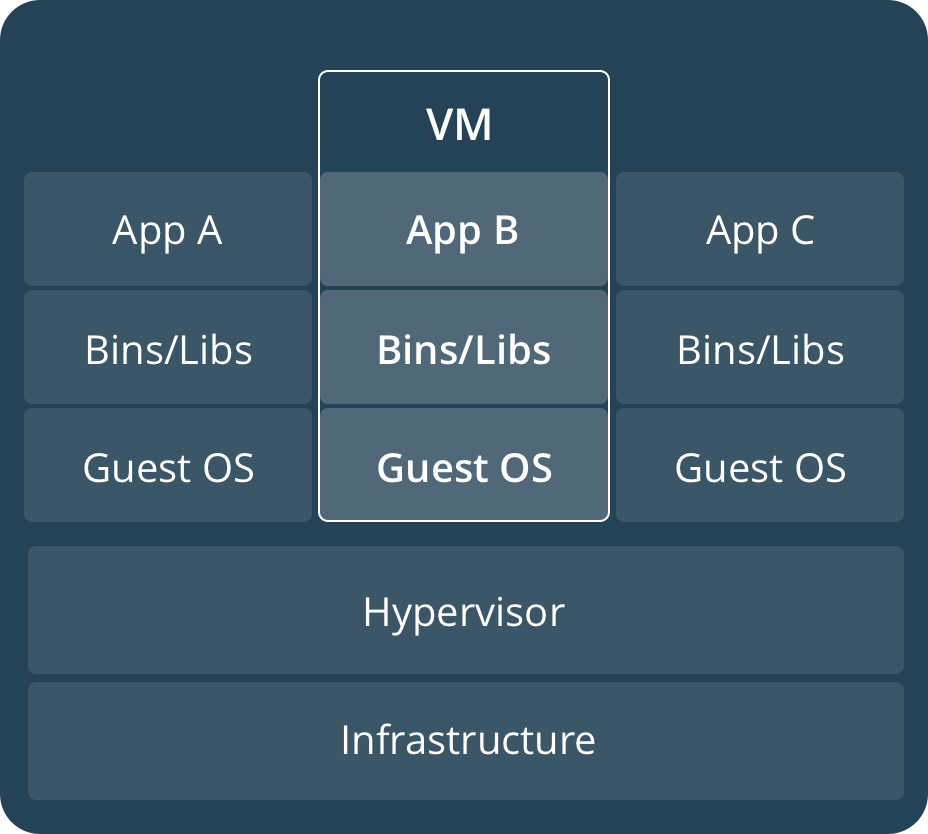
\includegraphics[width=.45\linewidth]{images/vm.png} }}%
	\quad
	\subfloat[Docker container]{{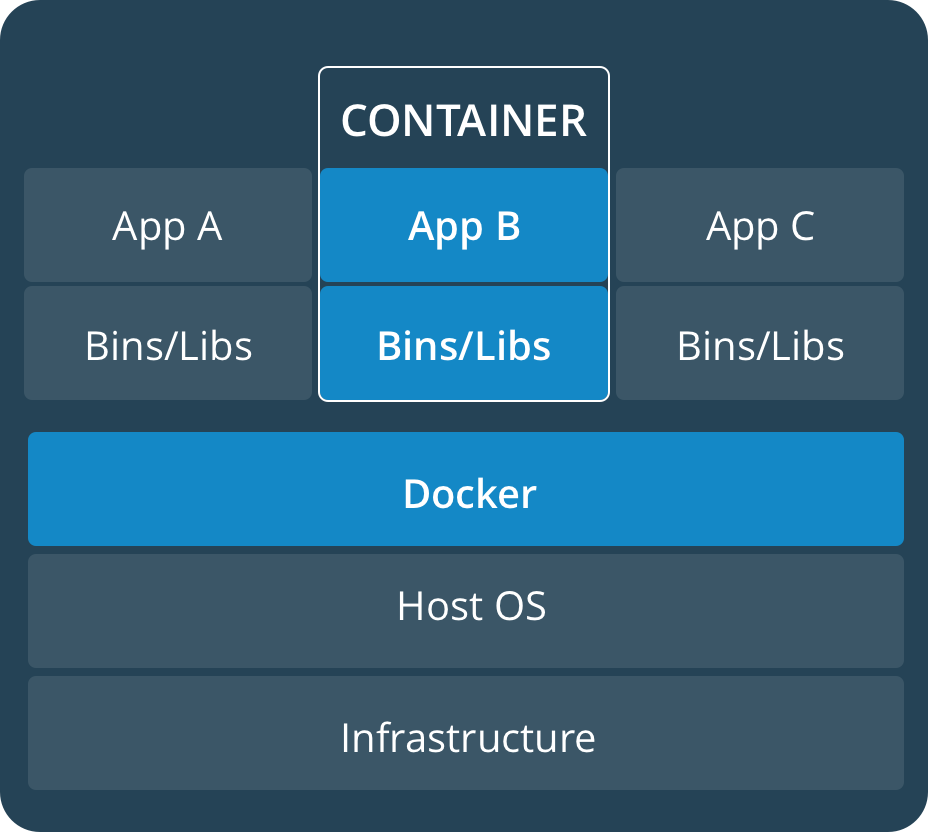
\includegraphics[width=.45\linewidth]{images/dockerContainer.png} }}%
	
	\caption{Comparison between hypervisor-based virtualization and Docker \cite{dockerdocu}}
	\label{fig:docker}
\end{figure}

It is an open source project that was originally build from many preexisting technologies in order to provide a more efficient virtualization technique as opposed to VMs. The tools that were used are mostly part of the Linux kernel as for example control groups (cgroups), used to manage and orchestrate the resource usage of a group of processes. Together with namespaces, that provide means to make resources only visible to a set of processes, they build the basis to separate the executable units from each other. These units are called \textit{containers} and are executed by the docker host via the system's kernel, using features like cgroups, namespaces, linux security models and many others to ensure strict separation from the rest of the system. Defining the composition and behavior of such a container is being done with so-called images. They are the blueprint, from which multiple containers can be derived from encapsulating the predefined contents inside multiple, read-only filesystem layers. Containers have a thin, writable layer at their disposal which is ephemeral. For persistence, volumes can be used to share data between the host and the container environment. The layering system in docker strives to minimize redundancies by sharing identical layers between multiple images, keeping the overall storage needs low \cite{fink2014docker} \cite{morabito2015hypervisors}.

Docker has gained a lot of popularity over recent years and as an open source project, it has favored the creation of a large ecosystem around it. This makes the usage of docker much easier, since documentation, community help and tutorials are readily available. When packaging an application or a service inside an image, often dependencies and libraries need to be included. The large ecosystem makes this almost painless, since many, official and verified images already exist that can be used as a basis.

\subsubsection{OVS and OpenFlow}
Provisioning network functionality inside containers necessitates that the attachment of the containers to the rest of the network can be realized with as much automation as possible, and secondly with high performance. Attaching the containers to virtual switches is an essential step since these can guarantee both of these requirements. 

Open vSwitch is such a switch, using the Openflow protocol to be able to communicate with an SDN controller and thus provide programmability. Since Linux Kernel 3.3, it comes bundled in it and provides multi layer switches and additional tools for a consistent setup, configuration and monitoring. The documentation provides insight into the authors' vision of what its main purpose is: Making networking easier in multi-server deployments that heavily rely on virtualization. In support of this high-reaching goal are several design characteristics: Making the migration of entities in the network as easy as possible is one of the core advantages of VNFs and CNFs and is realized by allowing the migration of configuration with the associated host. Supporting automation of the network is the fact that OVS holds the state in a database (OVSDB) while supporting triggering events remotely. OVS supports the idea of separating network traffic logically by tagging the packets. Finally, high performance during the interplay of hard- and software is guaranteed by allowing the forwarding path of the bridges to use the in-kernel datapath and directly communicating with the network interface cards (NIC). This also allows for simultaneous management of physical and software networking entities with the same technology. 

Figure \ref{img:ovs} shows how the different components of OVS interact. The OVSDB is located at the user space level and stores all the information about the virtual switch. Its contents are accessible via the SDN controller in the network, or the ovs-server.
Realizing the actual switch is the ovs-vswitchd daemon, located in user space. Communication and manipulation is being realized via the OpenFlow protocol and the Southbound API of the SDN controller. 
\cite{openvswitch} \cite{pfaff2015design}. 

\begin{figure}[h]
	\centering
	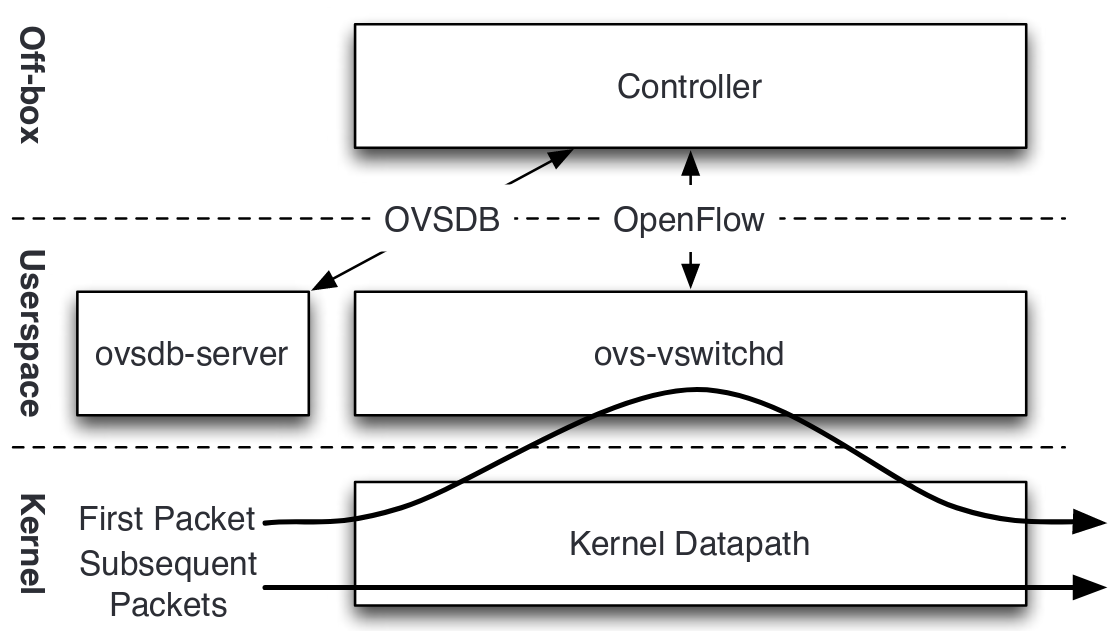
\includegraphics[width=1\linewidth]{images/openvswitch.png}
	\caption{Components and interfaces of Open vSwitch, source \cite{pfaff2015design}}
	\label{img:ovs}
\end{figure}

The OpenFlow protocol was developed in an educational environment by McKeown \textit{et al.} \cite{mckeown2008openflow} in 2008. Its main focus was to allow researchers to conduct experiments in their networks, while being "[...] open, vendor neutral, control-data plane interface [...]" \cite{berde2014onos}. Realizing its potential, the Open Networking Foundation (ONF) has adopted management and supports the extension and further development of OpenFlow.

\newpage
In traditional forwarding switches packets are being registered from the ports they arrive. Following that, they are analyzed, and from the information in the packets' header specific rules for how to deal with them are learned. The inner workings of this behavior are transparent to the user without a possibility to modify or extend. In contrast, OpenFlow provides a possibility to manipulate so-called flow tables, that represent the rules of how to deal with incoming packets. 
Figure \ref{img:of} shows such a flow table that prescribes what to do with incoming packets as prescribed by the SDN controller. For each packet, a rule will be looked up from top to bottom which will determined the behavior exactly. Information that can be used to match are various, like for example the MAC and IP addresses, port information and many others. In the figure these fields are marked in white color. The first column in gray prescribes what to do with a certain packet. For instance if a packet is destined to TCP port 25, it shall be dropped. Wildcards can be used and if nothing matches, the last line says to send the packet to the controller. Finally, the last column shows another advantage: Metrics for analysis of how often a rule has been applied. 
\cite{mckeown2008openflow}. 

\begin{figure}[h]
	\centering
	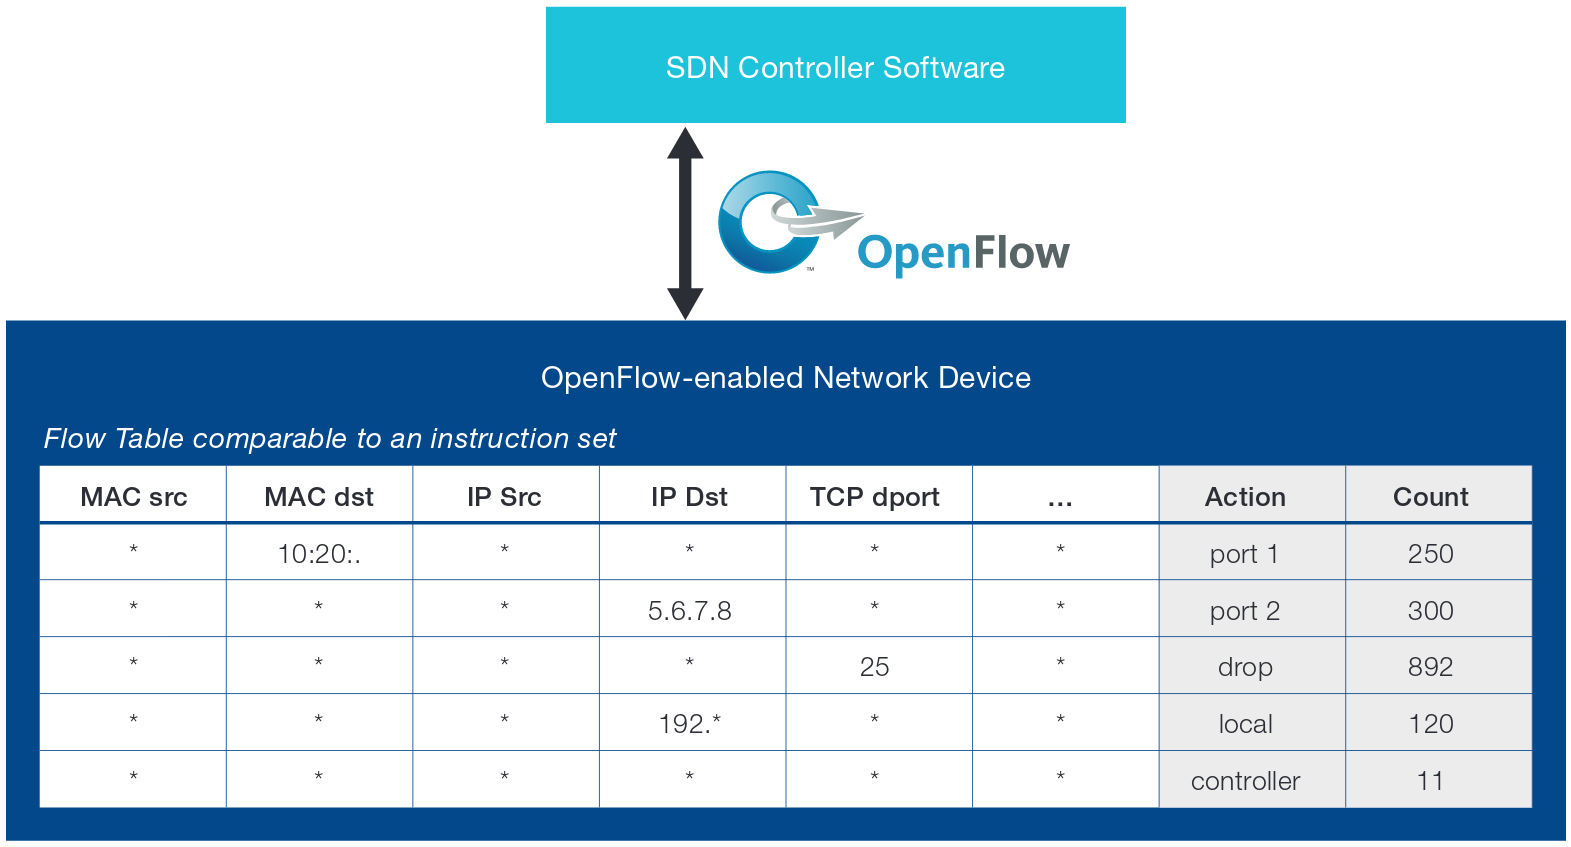
\includegraphics[width=1\linewidth]{images/of.png}
	\caption{Example of OpenFlow Instruction Set, source \cite{ofWhitePaper}}
	\label{img:of}
\end{figure}

This matching information can be manifold and includes but is not limited to the MAC/IP addresses of the sender or the receiver, the incoming port etc. In Figure \ref{img:of} these fields can be found on the left and are marked in white color. The two fields on the right serve a different purpose. The entry in the \textit{Action} column specifies what needs to be done to the packet if it conforms to the specified criteria. In this example it will either be output via port 1 or 2, dropped if it is directed at a TCP destination port 25, sent to local for processing if the IP destination starts with 192 or sent to the controller if no other rule applies. 

\subsubsection{Kubernetes}
All in all, the combination of these technologies renders unforeseen automation possible, especially in the network domain. When deploying functionality bundled in containers however, interacting directly with the Docker hosts on each compute node for each deployment is very cumbersome. There is the need for a system that manages multiple hosts, provides lifecycle management, load-balancing and scaling. 

Kubernetes is such a system that was developed by Google for its internal needs. The motivation was the handling and usage of Linux containers and the need arose for a management system. Since non existed, the company started developing its own. After building Borg and Omega as closed source systems, Kubernetes is an open source project and can be used in different environments, best known is Google's own public cloud service.

\begin{figure}[h]
	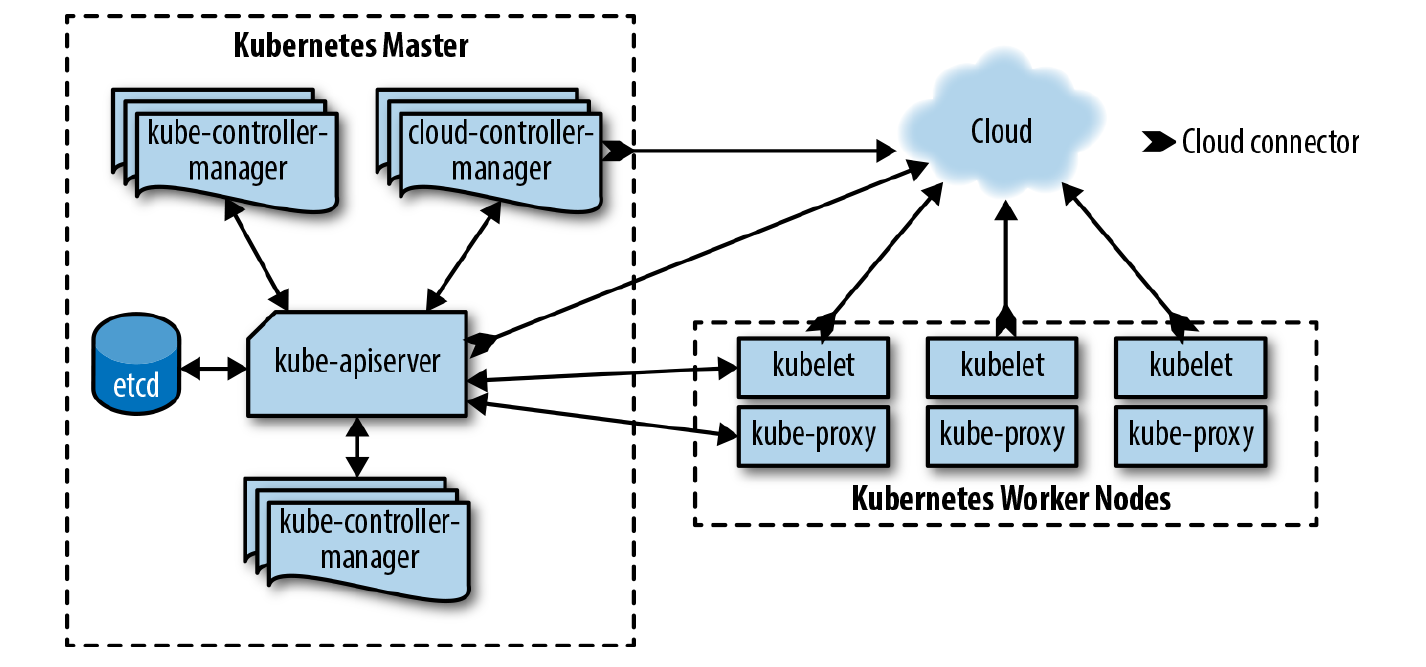
\includegraphics[width=\linewidth]{images/k8Arch.png}
	\caption{Kubernetes Components and their relationship \cite{k8CN}}
	\label{fig:k8}
\end{figure}

Figure \ref{fig:k8} summarizes briefly the components of the orchestration system that manages a cluster. One master manages multiple worker nodes, and generally speaking is not available for application-specific workloads. The single processes doing the orchestration are the following:

\setlength{\leftmargini}{0pt} 
\begin{description}
	\item [Kube-controller-manager] A daemon, managing several different controllers who know the desired state of the cluster and try to converge the real, observed state towards it. Each controller serves a different domain and has a defined set of responsibilities. Examples are the replication, endpoints, namespace and service accounts controller.
	
	\item [Kube-scheduler] This process manages the deployment of defined pods that bundle the execution of one or more containers to worker nodes inside the cluster. In order to make a sensible selection, the scheduler needs to know the resource usage of the worker nodes. Additional constraints that might be specified by the user have to be taken into account, too at this point. This is not explicitly included in figure \ref{fig:k8} but an essential part of the control plane.
	
	\item [Kube-apiserver] Central to the management of such a highly distributed system is the communication, which is served via JSON over HTTP. Validation and serving of API requests are the scope of work of this component. 
\end{description}

Apart from these processes, the manager needs to save the state of the cluster with all relevant information. This is being done in etcd and accessed by the kube-apiserver. The work for controlling the cluster is typically spread over multiple master-nodes to increase fault tolerance and ensure high availability. The etcd database containing the state of all the nodes and the deployments is also replicated and can survive individual failures in the control plane. 
The worker nodes in the cluster are there to provide an environment to execute application specific units. Therefore, a container runtime needs to be set up to start, monitor and stop containers. The process that enables this functionality on the worker nodes is called a kubelet. Ensuring communication not only within the cluster, but also with the rest of the attached network is the kube-proxy. When a worker node fails, the control plane will react to this event and try to mitigate the impact on the overall deployment automatically and ensure availability. Diverting the workload to other worker nodes is naturally only feasible as long as resources are still available in the cluster.

To sum up, Kubernetes provides a comprehensive management and orchestration framework for containerized applications. A unified approach to orchestrate, manage the lifecycle and monitor the status facilitates the cloud deployment. The general layout of the system is highly distributed and allows the usage of an overlay-network using Open vSwitch. This ensures that high networking performance and flexibility that is needed when building carrier-grade network functions. Additionally, the switches can be managed remotely via an SDN controller \cite{k8CN} \cite{burns2016borg} \cite{kubernetesUp}.

\subsubsection{Cloud-native paradigm}
%OVS switches, SDN and Openflow allow for unprecedented possibilities to automate network setup and orchestration. This  
Software engineering practices have moved in recent years from monolithic approaches towards a microservice architecture \cite{chowdhury2019re}. The main characteristic and motivation behind this shift is manifold: Making software more compartmentalized ensures a loose coupling that allows for easier development and upkeep of complex applications. These advantages prescribe the adherence to certain design principles to fully exploit them. 
Developers at Heroku, especially Adam Wiggins, have summarized these principles into the twelve factor methodology that takes into account the distributed environment of the cloud. Their methodology is cloud provider agnostic and helps guide developers towards building software on such a high level of abstraction where automation is key. The 12 factors are as follows:

\setlength{\leftmargini}{0pt} 
\begin{description}
	\item[Codebase] When developing an application, it is paramount to avoid fragmentation and keep everything in revision control (e.g. GIT). From one codebase, all the deploys, such as testing or production environments should be started. This ensures reproducibility and reduces the complexity. If multiple repositories with different codebases exist, each can be twelve factor app compliant and together they would form a distributed system.
	\item[Dependencies] An automated approach that creates an executable software fragment needs to have explicit access to all dependencies needed and thus developers have to declare them. This ensures unproblematic deployment in the target environment since assumptions about the existence of dependencies are forbidden. 
	\item[Config] Since there is only one codebase, but multiple deploys on possibly heterogeneous systems, manipulating certain behavior is necessary. This has to be solved by storing configuration in the respective environment. Often configuration variables are stored in constants inside the codebase, which does not allow to make adjustments without the need for rebuilding the complete application. This can be avoided by considering a deployment as bringing together a build artifact and configuration on an execution environment.
	\item[Backing services] All related services that are being used need to be treated as resources and thus be detachable and attachable. This allows swapping out services like database for instance without having to adapt the code. 
	\item[Build, release, run] For each stage, build, release and run, a strict separation needs to be ensured as to not introduce unforeseen behavior. Running a load test against the production environment could be detrimental to the user experience for instance. 
	\item[Processes] The application shall be realized as a set of stateless processes ensuring proper loose coupling and no side effects. Persistence should be organized with attached resources/services, for instance a remote database. For caching purposes however, using the local file system is acceptable. When a cloud function for instances needs to process a large image in multiple steps, it can use the local filesystem. The results need to be persisted appropriately to not be lost.
	\item[Port binding] Inter-service communication is very important and should be realized via listening on exposed ports. The underlying thought is making the twelve factor app completely self-contained. By relying on port-based communication, each app can become the backing service of another by declaring its URL in the configuration of possible consumers. 
	\item[Concurrency] Since the application should be built as an accumulation of stateless processes, scaling can be realized by horizontal replication.
	\item[Disposability] The single processes have to be disposable. Additionally, setup and teardown should be quick to realize to ensure robustness. 
	\item[Dev/prod parity] Developing in an environment that is as close to the actual production environment as possible ensures easier deployments and minimizes unanticipated behavior.
	\item[Logs] Logging is essential to debug an application and monitor it during execution. All processes treat logs as event streams and use \textit{stdout} and \textit{stderr} to facilitate aggregation by the execution environment. 
	\item[Admin processes] Tasks of administrative nature (e.g. database migration) should be executed as one-off tasks and kept close the application sources to ensure reproducibility.
\end{description}
\newpage
When an application is developed from the ground up with this methodology in mind, it can be called cloud-native. It should be clear by now that simply deploying a monolithic, classical application inside a VM or a single container is possible, but not appropriate for the cloud environment since its advantages can not be fully exploited \cite{hofmann2017microservices} \cite{12Factor}.

\begin{comment}
	
\begin{figure}[h]
	\centering
	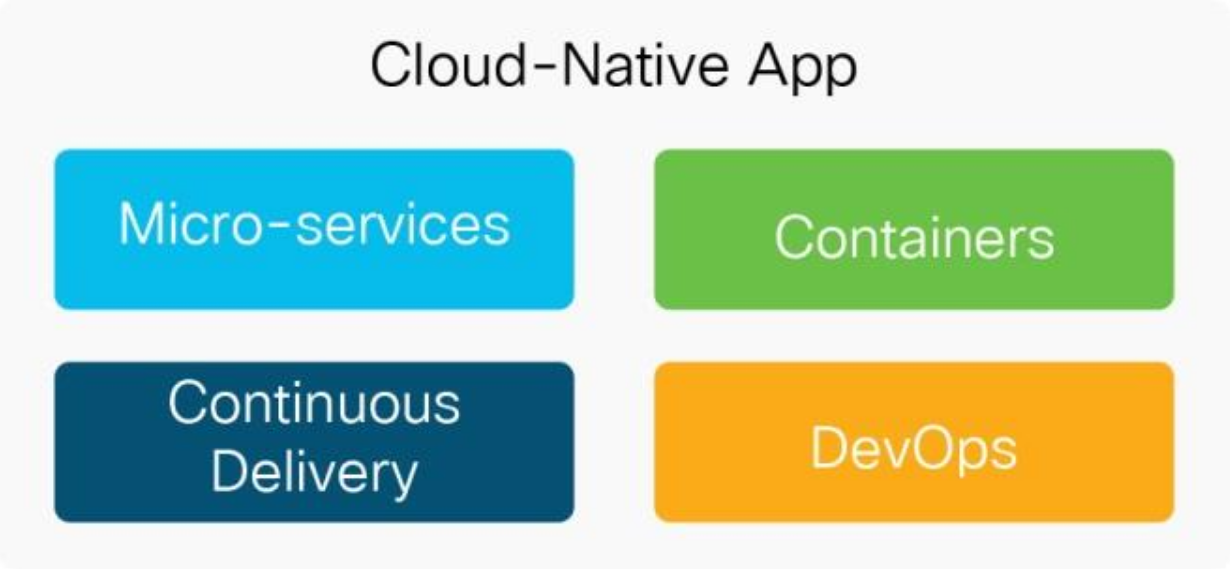
\includegraphics[width=0.75\linewidth]{images/cloudNativeApp.png}
	\caption{The principals of a cloud-native application as defined by the CNF \cite{CNF}}
	\label{img:cloudNativeApp}
\end{figure}
\end{comment}



\subsection{CNFs}
Powerful concepts have been introduced that can be used for different purposes when designing a network function that should conform to the cloud native paradigm: Containerization as an alternative concept to more heavyweight, hypervisor based virtualization. Orchestration and management of containerized services can be accomplished by Kubernetes that takes care of multiple issues: Deployment, lifecycle management, fault-tolerance, scaling and load-balancing. The Network Function Virtualization Infrastructure, responsible for providing an environment to deploy VNFs, can for instance be realized by using Kubernetes internally. Making use of the clustering concept ensures that the abstraction from multiple, physical compute nodes can happen seamlessly while ensuring their efficient usage. Management and monitoring functionality is well documented and built in, reducing the complexity of the Virtualized Infrastructure Managers. Their role shifts towards managing and monitoring the Kubernetes clusters available. Ensuring dynamic and flexible interconnection of the different components on the physical, as well as the virtual level can be accomplished with SDN and the switches under its domain. Open vSwitches and OpenFlow provide an easy and high performance way of interconnecting the different components dynamically. 

Realizing this vision is in the scope of Cloud-native Network Functions. When NFV was proposed by ETSI in 2012 in a white paper, no stable release for Docker and Kubernetes was in existence. The status quo were a plethora of physical middleboxes providing specialized functionality and the cloud had not the importance it holds today. Even so, cloud-native principles can be recognized in identified challenges of the document. Portability between several hardware vendors and different virtualization realization (e.g. hypervisors) had been identified. Management and Orchestration and automation efforts are central to scalability and profitable operations. The idea of building systems that can tolerate partial failures and are robust is still important to cloud native application development.
In the 2017 revision of the white paper, ETSI explicitly picked up the CNF concept. The additional benefit, especially in delimitation to VNFs is the fact that the functions are designed from the ground up with the execution in a cloud environment in mind. Further moving from monolothic software entities towards highly modular microservices that can be managed and scaled independently are of the highest priority.

The acceptance of this new paradigm is steadily rising, various vendors and initiative explore its possible usage scenarios and propose ways of adapting it on various abstraction levels (i.e. from high level architectures to actual products). 
The 5G-PPP (5G Infrastructure Public Private Partnership) initiative for instance has released a white paper titled \textit{From Webscale to Telco, the Cloud Native Journey} \cite{5gppp} that specifically tries to apply the experiences and best practices gathered in the cloud application engineering to the networking domain. The self-proclaimed goal is to ``[\dots] avoid the risk that 5G remains a niche connectivity gap-filler largely ignored by cloud applications and services boom'' \cite{5gppp}. The risk stems from the fact that this technology is very expensive, and can only become profitable when the new possibilities are fully taken advantage of. This entails providing end-to-end services on a per-customer basis, which poses considerable challenges. These can only be achieved, when fully embracing all the previously mentioned concepts and taking them into consideration when designing both, the Virtualized Network Functions, as well as the infrastructure they are supposed to be deployed to \cite{5gppp}.

% Implementations NFV4ARM
\begin{figure}[h]
	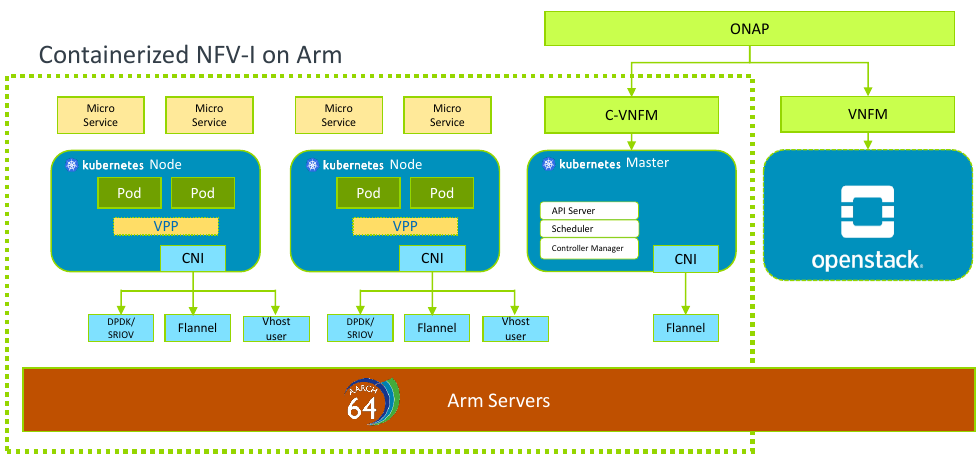
\includegraphics[width=\linewidth]{images/nfv4arm.png}
	\caption{ONAP extension for NFV on ARM \cite{nfv4arm}}
	\label{fig:nfv4arm}
\end{figure}

Implementing the Cloud-native Network Function (CNF) functionality in orchestrator software already exists and can serve to showcase how this can be realized. An extension to the Open Network Automation Platform (ONAP), part of the Linux Foundation that exposes a southbound API to communicate with a NFVI/VIM, can be seen in figure \ref{fig:nfv4arm}. This is a hybrid model since over the southbound API a classical VNF Manager (VNFM) is attached that uses Openstack to manage virtual machines and additionally, a Containerized-VNFM has been registered to the automation platform. This manager coordinates the CNF deployment via directly via the Kubernetes master node, that is in charge of the different worker nodes.


\begin{comment}
	“Lift and shift” architectures brought certain benefits of virtualization, mostly related to the fact that
	the hardware can be shared between different functions. However, they did not solve issues related to scaling, feature velocity and availability because the code was still a monolith captured in a VM.
	Cloud native (which encompasses the three disciplines mentioned above) is a re-design of the
	network functions themselves.
	Current cloud native systems are focused on managing enterprise and web commerce, not packet
	forwarding. The purpose of this paper is to show that all the issues related to building a cloud native
	NFVs are solvable problems. The design principals that made cloud native a success can be applied
	to network function virtualization as well, driving the same service velocity, availability and scaling
	to the networking world.
	
	cloud native network function virtualization true cloud for nfv
\end{comment}



\begin{comment}

\begin{figure}[h]
	\centering
	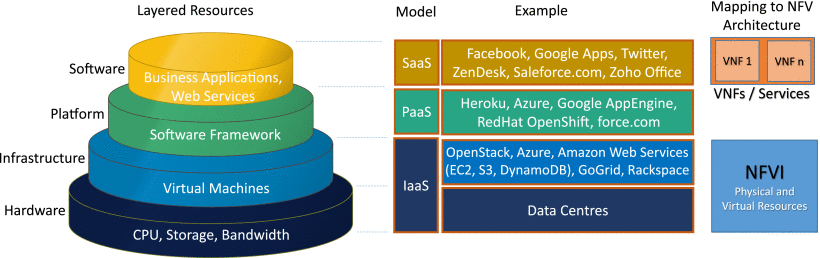
\includegraphics[width=1\linewidth]{images/arch.png}
	\caption{This is the caption \cite{mijumbi2016network}}
	\label{img:arch}
\end{figure}

\end{comment}